\documentclass{article}
\usepackage[utf8]{inputenc}
\title{Video 2: Principal Component Analysis}
\author{wbg231 }
\date{December 2022}
\newcommand{\R}{$\mathbb{R}$}
\newcommand{\B}{$\beta$}
\newcommand{\A}{$\alpha$}
\newcommand{\D}{\Delta}

\newcommand{\avector}[2]{(#1_2,\ldots,#1_{#2})}
\newcommand{\makedef}[2]{$\textbf{#1}$:#2 }
\usepackage{tikz,graphicx,hyperref,amsmath,amsfonts,amscd,amssymb,bm,cite,epsfig,epsf,url}

\begin{document}

\maketitle

\section{introduction}
\begin{itemize}
\item \href{https://www.youtube.com/watch?v=l9qIW_UBiZs}{vedio link}
\item today we are talking about pca 
\subsection*{motivation}
\item our goal is describe data with multiple features.
\item we mode our d-dimensional data set as a random vector $$\Tilde{x}=\begin{pmatrix}
    \Tilde{x}_1\\..\\\Tilde{x}_d
\end{pmatrix}\in \mathbb{R}^{d}$$
\item our idea is to find the directions in which our random vector has the most variance 
\subsection*{projection in a certain direction}
\item recall from the last Video what the how we compute the variance of a random vector $\Tilde{x}$ in the direction of unit vector $b\in \mathbb{R}^{d}$ we do this by projecting x onto b that is $P_{b}(\Tilde{x})=\frac{b^{t}\Tilde{x}}{||b||}=b^{t}\Tilde{x}$
\item in general we can think of the random vector $\Tilde{x}$ as composed of a section which is colinear to the vector b and a section that is orthogonal to b that is $\Tilde{x}=P_{b}\Tilde{x}(b)+(\Tilde{x}-(P_{b}\Tilde{x})b)=(b^{t}\Tilde{x})(b)+(\Tilde{x}-(b^{t}\Tilde{x})b)$ where b has unit norm 
\item we write in this way due to the fact that the variance of any linear combination of the random $\Tilde{x}$ and a vector $b\in \mathbb{R}{d}$ can be expressed as $$var(b^{t}\Tilde{x})=b^t\Sigma_{\Tilde{x}}b$$ where $\Sigma_{\Tilde{x}}$ is the covariance matrix of $\Tilde{x}$
\item this allows us to consider the function $f:A\Rightarrow\mathbb{R}: A:=\{a\in \mathbb{R}^{d} : ||a||=1\}$ where
 $f(a)=var(a^t\Tilde{x})=a^{t}\Sigma_{\Tilde{x}}a$
\item plotted over the contour diagram of a certain gaussian random vector that function looks
 like this \\ 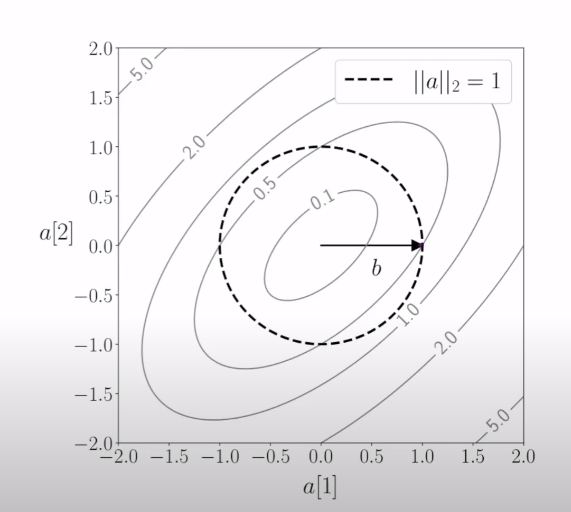
\includegraphics[width=5cm]{/home/buzgalbraith/work/school/spring_2023/probaility-theroy-2-2023/notes/week_8/vedio_2/immages/v2_1.png}
\item then plotting this in 2d as a function of radians looks like this 
 \\ 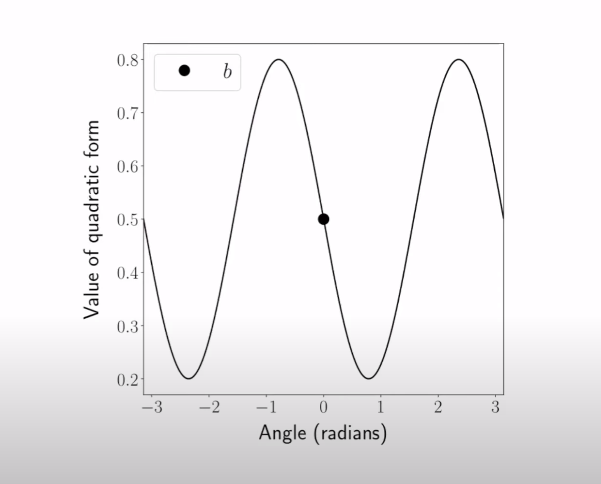
\includegraphics[width=5cm]{/home/buzgalbraith/work/school/spring_2023/probaility-theroy-2-2023/notes/week_8/vedio_2/immages/v2_2.png}
 \item so the direction of max variance in this case would be any point at the top that wave
 \item this expands to higher dimensional objects
 \item so now we want to know how we can find the optima in a more general sense. 
\subsection*{the spectral theorem}
\item given $M\in \mathbb{R}^{d\times d}$ is symmetric then it has an eigen decomposition 
\item $M=\begin{pmatrix} u_1 & u_2 & ...& u_d\end{pmatrix}\begin{pmatrix} \lambda_1 & 0 & ...& 0\\
    ..& ... & ...& ..\\
    0 & 0 & ...& \lambda_d\end{pmatrix}\begin{pmatrix} u_1 \\ u_2 \\ ... \\ u_d\end{pmatrix}=U\Lambda U^t=U\Lambda U^{-1}$
\item where the eigenvalues $\lambda_1\geq \lambda_2 \geq ... \geq \lambda_d$  (that is are sorted)
\item and eigenvectors $u_1...u_d$ are orthogonal 
\item and $u_i$ is the eigenvectors corresponding  to $\lambda_i$
\item and $U$ is an orthogonal matrix
\item we are going to go into this more next vedio
\item from this we see $\lambda_1=max_{||a||_{2}=1}a^tMa$ ie our largest eigenvalue is the maximal variance in any single direction
\item and $u_1=argmax_{||a||_{2}=1}a^tMa$ and our eigenvector corresponding to the largest eigenvalue is our direction of maximal variance
\item  then we can find the kth maximal direction of variance and it's associated variance orthogonal to our previous directions as $$\lambda_{k}=max_{||a||=1, a\perp u_1 \dots a\perp u_k}a^tMa, \quad \forall k \in [2,d-1]$$
$$u_{k}=argmax_{||a||=1, a\perp u_1 \dots a\perp u_k}a^tMa, \quad \forall k \in [2,d-1]$$
\subsection*{showing covariance matrix is symmetric}
\item let $\Tilde{a}$ be an arbitrary random vector
\item we can define  the centered version of $\Tilde{a}$ as $\Tilde{x}:=\Tilde{a}-E[\Tilde{a}]$ 
\item so we can see that $E[\Tilde{x}]=E[\Tilde{a}-E[\Tilde{a}]]=E[\Tilde{a}]-E[\Tilde{a}]=0$
\item and $var(\Tilde{x})=var(\Tilde{a}-E[\Tilde{a}])=E[(\Tilde{a}-E[\Tilde{a}] - E[\Tilde{a}-E[\Tilde{a}]])^2]=E[(\Tilde{a}-E[\Tilde{a}]])^2]=var(\Tilde{a})=\Sigma_{\Tilde{x}}=\Sigma_{\tilde{a}}$
\item so this just is saying can take an arbitrary random vector and center it to have mean 0 and the same variance
\item now we want to show $\Sigma_{\tilde{x}}=\Sigma_{\tilde{x}}^{T}$
\item we know that $\Sigma_{\Tilde{x}}=var(\Tilde{x})=E[(\Tilde{x}-E[\Tilde{x}])^2]=E[(\Tilde{x})^2]=E[\Tilde{x}\Tilde{x}^{t}]$
\item so thus $\Sigma_{\Tilde{x}}^{t}=(E[\Tilde{x}\Tilde{x}^{t}])^{t}=E[(\Tilde{x}\Tilde{x}^{t})^{t}]=E[(\Tilde{x}\Tilde{x}^{t})^{t}=E[\Tilde{x}\Tilde{x}^{t}]=\Sigma_{\Tilde{x}}$
\item so yeah the covariance matrix is symmetric, and thus we can use the spectral theorem
\subsection*{Principal directions}
\item let $u_1..u_d$ be the eigenvectors of $\Sigma_{\Tilde{x}}$ and $\lambda_1...\lambda_d$ be there corresponding eigenvalues
\item from this we see $\lambda_1=max_{||a||_{2}=1}a^tMa=max_{||a||_{2}=1}var(a^tM)$ ie our largest eigenvalue is the maximal variance in any single direction
\item and $u_1=argmax_{||a||_{2}=1}a^tMa=argmax_{||a||_{2}=1}var(a^tM)$ and our eigenvector corresponding to the largest eigenvalue is our direction of maximal variance
\item  then we can find the kth maximal direction of variance and it's associated variance orthogonal to our previous directions as $$\lambda_{k}=max_{||a||=1, a\perp u_1 \dots a\perp u_k}a^tMa=max_{||a||=1, a\perp u_1 \dots a\perp u_k}var(a^tM), \quad \forall k \in [2,d-1]$$
$$u_{k}=argmax_{||a||=1, a\perp u_1 \dots a\perp u_k}a^tMa=argmax_{||a||=1, a\perp u_1 \dots a\perp u_k}var(a^tM), \quad \forall k \in [2,d-1]$$
\item we can call $u_{i}$ the ith Principal direction of $\Tilde{x}$
\item so back to this graph \\ 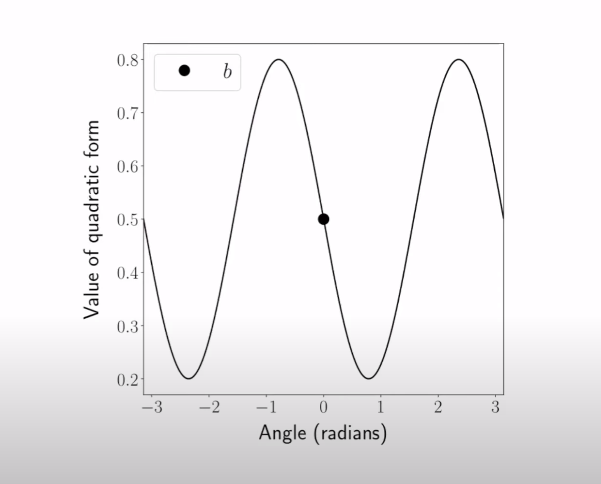
\includegraphics[width=5cm]{/home/buzgalbraith/work/school/spring_2023/probaility-theroy-2-2023/notes/week_8/vedio_2/immages/v2_2.png}
\item we know that our function will be maximized at the first Principal direction (the first eigenvector of the covariance matrix of $\Tilde{x}$)
\item looking at the joint pdf of our random vector we can indeed see that the first Principal direction does capture the most variance graphically \\ 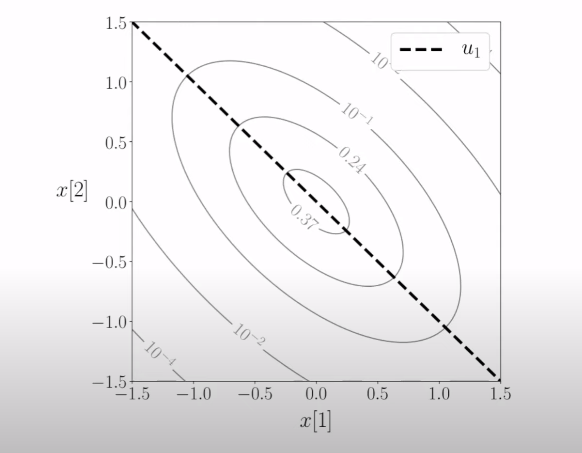
\includegraphics[width=5cm]{/home/buzgalbraith/work/school/spring_2023/probaility-theroy-2-2023/notes/week_8/vedio_2/immages/v2_3.png}
\item we can naturally find the minimum variance direction by just looking for the eigenvector associated with the minimum eigenvalue
\subsection*{Principal Components}
\item let $ct(\Tilde{x})=\Tilde{x}-E[\Tilde{x}]$ be our centered random vector
\item the \textbf{Principal Component} corresponding to each \textbf{Principal direction} is defined as 
$$\Tilde{w}_{i}=u_{i}^{t}ct(\Tilde{x})= P_{u_{i}}ct(\Tilde{x})\quad \forall i\in [1,d]$$ that is the inner product between our centered random vector $ct(\Tilde{x})$ and the Principal direction $\Tilde{u}_{i}$ or in other words our random vector projected onto that Principal Component
\subsection*{variance of the ith Principal Component}
\item $var(\Tilde{w}_{i})=var(u_ict(\Tilde{x}))=u_i^{t}\Sigma_{ct(\Tilde{x})}u_i=u_i^{t}\Sigma_{\Tilde{x}}u_i=\lambda_i u_i^{t}u_i=\lambda_{i}||u_1||=\lambda_i$ since our eigenvector are unit norm 
\item recall that by spectral theorem these variances correspond to the variance in the ith Principal direction that is $$\lambda{i}=max_{||a||_2=1, a\perp u_1,\dots, a\perp u_{i-1}}var(a^t\Tilde{x}_{i})=var(\Tilde{w}_i)=var(u_ict(\Tilde{x})), \quad \forall i \in [2,d]$$
\item so this goes to show that our definition of Principal Components result in Components that have maximal variance
\subsection*{example}
\item so for a certain gaussian random vector $\Tilde{x}\in \mathbb{R}^{2}$
\item we say can plot it's first Principal direction as \\ \includegraphics*[width=4cm]{/home/buzgalbraith/work/school/spring_2023/probaility-theroy-2-2023/notes/week_8/vedio_2/immages/v2_4.png}
\item then computing the corresponding first Principal Component as $\Tilde{w}_i=u_i^{t}ct(\Tilde{x})$ and plotting its pdf    \\  \includegraphics*[width=4cm]{/home/buzgalbraith/work/school/spring_2023/probaility-theroy-2-2023/notes/week_8/vedio_2/immages/v2_5.png}
\item this tells us that the first principal component of our gaussian random vector is a gaussian random varibale is a gaussian with fairly high variance
\item as this is only a 2 dimensional random vector we know it's other principal direction will be the direction of minimal variance graphing this we see \\  \includegraphics*[width=4cm]{/home/buzgalbraith/work/school/spring_2023/probaility-theroy-2-2023/notes/week_8/vedio_2/immages/v2_6.png}
\item and plotting the pdf of the second principal Component we get \\ \includegraphics*[width=4cm]{/home/buzgalbraith/work/school/spring_2023/probaility-theroy-2-2023/notes/week_8/vedio_2/immages/v2_7.png} 
\item which is good as we can see the second Principal Component of our random vector is a gaussian random variable with lower variance
\item now we can look at the joint pdf of our two Principal Components $\Tilde{w}_1, \Tilde{w}_2$ \\  \includegraphics*[width=4cm]{/home/buzgalbraith/work/school/spring_2023/probaility-theroy-2-2023/notes/week_8/vedio_2/immages/v2_8.png}
\item this graph makes sense as we are centering our data (then rotating it in the direction of our Principal Components) so that we have the ellipse that are most spread out in the first dimension and least spread out in the second 
\item this also leaves us with uncorrelated Component
\subsection*{corelation}
$E[\Tilde{w}_{i}\Tilde{w}_{j}^t]=E[(u_i^{t}ct(\Tilde{x}))(u_j^{t}ct(\Tilde{x}))^{t}]=E[u_i^{t}ct(\Tilde{x})ct(\Tilde{w})u_j]=u_i^{t}E[ct(\Tilde{x})ct(\Tilde{x})]u_j=u_i^{t}\Sigma_{\Tilde{x}}u_{j}=\lambda_{j}u_i^{t}u_{j}=0$
\item so from this we get $var(\tilde{w}_{i}+\tilde{w}_{j})=var(\Tilde{w}_{i})+var(\Tilde{w}_{j})-2cov(\Tilde{w}_{i}\tilde{w}_{j})$ this shows that these two Components are orthogonal
\item $cov(\Tilde{w}_{i}^{t}\Tilde{w}_{j})=E[\Tilde{w}_{i}^{t}\Tilde{w}_{j}]-E[\Tilde{w}_{i}]^{t}E[\Tilde{w}_{j}]$
\item $E[\Tilde{w}_{j}]=E[u_{i}^{t}ct(\Tilde{x})]=u_i^{t}E[ct(\Tilde{x})]$
\item $cov(\Tilde{w}_{i}^{t}\Tilde{w}_{j})=E[\Tilde{w}_{i}^{t}\Tilde{w}_{j}]-E[\Tilde{w}_{i}]^{t}E[\Tilde{w}_{j}]=0-(u_i^{t}E[ct(\Tilde{x})])^{t}u_j^{t}E[ct(\Tilde{x})]=E[ct(\Tilde{x})]^{t}u_iu_j^{t}E[ct(\Tilde{x})]=0$
\item going to show that $var(\tilde{w}_{i}+\tilde{w}_{j})=var(\Tilde{w}_{i})+var(\Tilde{w}_{j})-2cov(\Tilde{w}_{i}\tilde{w}_{j})=var(\Tilde{w}_{i})+var(\Tilde{w}_{j})$ and thus $\Tilde{w}_{i}, \Tilde{w}_{j}$ are uncorrelated
\subsection*{gaussian example}
\item the eigenvalues of a gaussian random vector's covariance matrix are the axis of it's contour lines (which are ellipses)
\subsection*{pca from data}
\item given a dataset $\mathcal{D}=(x_1...x_n) : x_i\in \mathbb{R}^{d}$
\item our steps of pca are 
\begin{enumerate}
    \item compute teh sample covariance matrix $\Sigma_{d}$
    \item take the eigen decomposition of $\Sigma_{X}$ which yields principal direction $u_1...u_d$
    \item center the data and compte the Principal components as $$w_j[i]=uj^{t}ct(x), \quad \forall i\in [1,d], j\in [1,d]$$ where $ct(x_i)=x_i-M(x)$ so we are projecting the data onto the Principal Components
\end{enumerate}
\item this is optimal with respect to sample variance
\subsection*{example}
\item data set with latitude and longitude of cities 
\item have data set $x=\{x_1...x_n\}$
\item projecting our data onto direction a  is given by $X_{a}:=\{a^tx_1...a^tx_n\}$
\item we know that the sample variance of $X_a$ is given by $v(X_a)=a^t\Sigma_X a$ we showed in last Video this gives us exactly the sample variance
\item we can again show that the Principal Components are the exact directions of maximal sample variance for our dataset by the exact same logic as what we did in the random vector case. 
\subsection*{other example}
\item here we are looking at a dataset of face immages where each image $x_i\in \mathbb{R}^{64\times 64}$ then we are going to flatten those to vector such that $x_i\in \mathbb{R}^{4096}$
\item now we can build a covariance matrix $\Sigma_{x}\in \mathbb{R}^{4096\times 4096}$ and taking the eigenvectors of that we get the principal direction which we can then project the data onto to get the Principal Component $u_1...u_{4096}$
\item here are the first few Principal components \\ \includegraphics*[width=5cm]{/home/buzgalbraith/work/school/spring_2023/probaility-theroy-2-2023/notes/week_8/vedio_2/immages/v2_9.png}
\item here are some lower Principal Components few Principal components \\ \includegraphics*[width=5cm]{/home/buzgalbraith/work/school/spring_2023/probaility-theroy-2-2023/notes/week_8/vedio_2/immages/v2_10.png}
\item we can see that the higher principal Components capture some of the course features of our data like nose or glasses 
\item the lower Principal Components are more fine and often give us less interpretable features 
\end{itemize}
\end{document}
